\section{Features}
\label{sec:features}
This section defines the features used in the implementation of Learn to Rank algorithm. All features are summarized in table \ref{features_tab} and described in the following sections.

\subsection{Link Position}
\label{link position}
\paragraph{Description.}
Position of a link in an article is the number of characters counted from the beginning of the article up to the link appearance. Because the length of different articles may vary quite substantially, this number is normalized per article. Second variant takes logarithm of link position and normalizes it per article.

\paragraph{Motivation.}
Our intuition behind the Link Position feature is based on two observations. The first one is that given the way Wikipedia articles are structured, the most general description of the article is placed in the first few paragraphs before the table of contents. This section of the Wikipedia article is called the lead section \cite{lead}. As described in the Wikipedia manual of style, for many people, the lead section is the only section they will read since it summarizes the entire article. Later paragraphs only dive deeper into the topics outlined in the description. 

The second observation is the way people read web pages. As explained in \cite{nielsen} by Jakob Nielsen, one of the leaders in human-computer interaction, on average, users have time to read at most 28 \% of the words on a website. Additionally, most attention is given to the top portion of a page and later sections are merely skimmed through. People looking for different article that is somewhat related to the one currently being read might be interested in more general concepts as they contain the searched term. %As explained above, more general terms happen to be heavily abundant in the top portion of a Wikipedia article.

\paragraph{Extraction.}
Raw texts of the articles in Wiki markup are taken from the Wikipedia dumps described above and links to other articles are found using regular expressions. Links to images, external sources, etc. are ignored. Due to the nature of source from which is this feature extracted, there might be slight discrepancies in position value and the exact number of characters preceding the links in final article as displays in web browser.

\subsection{Link Order}
\label{link order}
\paragraph{Description.}
This feature captures the position of a link relative to all the other links contained in the same article. The order equal to $n$ means that the link is the $n^{th}$ link in the article. The final value of this feature is again normalized per article. Second variant takes logarithm of link order and normalizes it per article.

\paragraph{Motivation.}
Similar to the previous feature, Link Order is based on the observation that a Wikipedia article's initially describe the topic in general terms. While the link position captures more of a distance between links and their spread, link order is a simplified version of it. It conveys less information, but in a much more straightforward manner.

\paragraph{Extraction.}
This feature is also extracted from the Wikipedia dumps in a similar manner to the Link Position feature.

\subsection{Link Count}
\label{link count}
\paragraph{Description.}
Link Count is the number of occurrences of the same link throughout the article.

\paragraph{Motivation.}
Whenever a link is present multiple times in a single article, it means that the topic is repeated several times in the article as well. This may signify strong relatedness of the article's content.

\paragraph{Extraction.}
The feature is extracted from the Wikipedia dump using the raw article texts as in case of the previous two features.

\subsection{Popularity of Resource}
It seems reasonable to assume that users have a tendency to click on links to articles that are describing trending and popular topics. This is the motivation for constructing the feature described in details below where a numerical measure is estimating a degree of user interest for the resource article $\beta$ in the pair $(\alpha, \beta)$. \\

For our model to be applicable to new articles, we should not, in general, use any information on article $\alpha$ that are caused by user behaviour. If we were to use this information we would not in practice be able to apply our model to new articles before sufficient data has been logged. 


\subsubsection{Description}
From the clickstream data it is possible to derive the number of article views on a an article that are as a result of external traffic i.e. traffic coming from outside the Wikipedia domain. This gives the possibility of extracting the number of searches from known search providers: Google, Bing and Yahoo! or the number of visits from social media sites such as Twitter and Facebook. This is traced using the HTTP header information: `referer'. Note that this information is completely separated from the information used for creating the ground truth -- for that only internal click counts were used.\\

Furthermore we limit ourselves to using traffic data from external and well known sources and not include data from internal Wikipedia searches or when the referrer is missing: This could possibly be due to spoofed referral headers which could introduce a bias to our model.\\

We consider traffic from search and social media individually as \fxnote{insert ref http://research.microsoft.com/pubs/154556/wsdm11-twitter.pdf} states that users might have different intentions depending on which media they choose to search or browse for content. Users on social media, unlike for search engines, tends to look for content that is currently trending.

\subsubsection{Extraction}
\fxnote{Nothing in this section makes sense right now}
Virality and derived measures for popularity originating from social networks usually follows a power law distribution as a consequence of the social network forming scale-free graphs. [1]

Assuming both search- and social media traffic are directly influenced by social networks we have an idea of the distribution of traffic to wiki articles from these sources. According to the power law this would mean that low-popularity articles are very common whereas high-popularity articles can be extremely rare.

Characteristic for a power law distribution is that the log-log plot of the probability density function (PDF) is linear. The below figure illustrates this. The articles considered is all distinct 𝛃-articles for all ɑ in A, i.e. all distinct prominent-linked articles.

We see that the popularity originating from search traffic of these mentioned articles follow a power law distribution.

Knowing the distribution of the click data from social medias and search we can preprocess the features including traffic volumes from these sources. An easy and effective way of coping with the non-linearity of the power law distribution is by taking the logarithm twice of the popularity ln( ln( beta ) ) and thereafter normalizing the feature values using the maximum value.
The final outcome of this processing results in the feature having a correlation coefficient of $r = 0,3879$ and a `coefficient of determination' of $r^2 = 0,15$.  

In the below figures the PDF is shown for the search volumes respectively without taking the log, with the log and with the log twice. The distribution of feature values `flattens out' and signs of any exponential growth or decay disappears.

For the above 3 tests we have a `coefficient of determination' of respectively 0,0045, 0,113 and 0,150, thereby effectively selecting the 3. option as an input feature for the model.

It must be noted for the cases where the popularity are zero, we simply skip preprocessing because of the nature of the logarithm.





\subsection{Popularity Percentile Rank}

\fxnote{the following is just raw notes}

Another feature to derive from clickstream data is for an instance pair $( ɑ , beta)$ where beta is in $B$ the probability that an arbitrary article $ɣ in B \ { beta }$ has a lower popularity than beta:
$f( ( ɑ , beta) ) = pr( pop(beta) > pop(ɣ) )$

Characteristic for this feature is that if $pop(beta)$ is the maximal value for any article in $B$, then the feature value gives:
$f( ( ɑ , beta_max) ) = 1$

If $pop(beta)$ is the minimum value for any article in $B$, then the feature value gives:
$f( ( ɑ , beta_min) ) = 0$

And if $pop(beta)$ is equal to the median value of the articles in $B$, where all article popularity values are distinct, then the feature value gives:
$f( ( ɑ , beta_med) ) = 0.5$

This feature gives an opportunity to extract more knowledge on the distribution of article popularity locally for a prominent article.

The coefficient of determination yields $r^2 = 0,0582$.

\subsubsection{Description}
x
\subsubsection{Motivation}
x
\subsubsection{Extraction}
x




\subsection{Title similarity}
\fxnote{Just raw notes - and it should be together with the other sim features}
A last feature to extract from the clickstream data is title similarity. This feature is fairly trivial and motivated by e.g. the observation that articles on people often have their family members among the most popular reference links and these often share familyname whereas we would observe a higher title similarity. The feature was implemented using a Jaccard similarity measure and normalized from 0 to 1. We achieved a coefficient of determination on $r^2 = 0,0115$.


\fxnote{INCOMPLETE} \\

\subsection{Community Membership}
\label{community membership}
\paragraph{Description.}
Let $G(V,E)$ be a simple graph. Then a community in $G$ is a subgraph $(V', E') = G' \subseteq G$, such that $|E'| \ge |\{ \{u,v\} \in E\setminus E'  \; | \; \{u, v\} \cap V' \neq \emptyset \}|$. In our case the $G$ is a graph of Wikipedia, where $V = \bigcup_{i=1}^{M} B_i \cup P$ is a set of articles and $E$ is set of links between them. After detecting all communities, each edge (link) $\{p_i,\beta_j\}$ is given a value of 1 if both $p_i$ and $\beta_j$ belong to the same community or 0 otherwise.

\paragraph{Motivation.}
Communities are an implicit clustering of articles on Wikipedia that capture emerging properties of interconnected articles. This feature looks promising in cases where someone is interested in a specific topic, be it music bands of the same genre or fields of study in a certain science. Related articles from the same community might be a good place to look at and will highly likely contain desired article. Furthermore, users reading an article have shown an interest in specific topic and might want to broaden and deepen his or her knowledge of it.

\paragraph{Extraction.}
Every link extracted from the Wikipedia dump is converted into an edge of a graph. The resulting graph is then loaded and communities are found using igraph package in R. Community detection algorithms used were Fast greedy \cite{fast_greedy}, Label propagation \cite{label_propagation}, and InfoMAP\cite{infomap}. The graph was transformed into a simple graph and then community detection algorithms were run. Even though links have natural orientation, one can relax them as undirected edges. Sheer number of links by it self is an adequate indicator of community belonging regardless of their orientation.

\subsection{Symmetric Linking}
\label{symmetric linking}
\paragraph{Description.}
A link $(p_i, \beta_j)$ is considered symmetric if, and only if $\beta_j \in B_i$ and link $(\beta_j, p_i)$ also exists. If the link is symmetric, the feature has a value of 1 and 0 otherwise.

\paragraph{Motivation.}
Symmetric linking indicates, in some cases, that there exists an important relevance between said articles or highly related topics are being discussed. Examples of this article relationship includes competing presidential candidates, sports team rivals, movies and its actors, etc. As expected, it is common for users to demonstrate interest in these kind of relations between articles.

\paragraph{Extraction.}
This feature is extracted from the Wikipedia dump file. First, all the links between prominent articles in $P$ and articles in all $B_i$ for $1 \le i \le M$ are found. Then for every link $(p_i, \beta_j)$ a link $(\beta_j, p_i)$ is looked up.

\subsection{HITS and PageRanks}
\label{hits and pagerank}
\paragraph{Description.}
HITS and PageRank characterize nodes in the graph by score based on number of edges and also the scores of neighbours.

Although HITS and PageRank differ in content their main goal is the same, give estimate of article significance. In case of HITS, high hub score may indicate more general topics while high authority score would be indication of very focused article discussing particular term in great depth. PageRank is similar to the hub and authority score combined.

\paragraph{Motivation.}
The intuition behind this feature comes from the search engine domain. When searching, these scores help identify the most relevant results. When applied to articles, the scores will help categorize linked articles for the learning to rank algorithm.

\paragraph{Extraction.}
Similarly to community extraction, HITS and PageRank are computed from graph representation of Wikipedia. The graph is processed in R using package igraph that implements both \cite{pagerank} and \cite{hits}. Link directions are preserved in this case.

\subsection{Relatedness obtained from links}
\label{relatedness obtained from links}
This feature measures how two articles are related in terms of linking. Indeed, it compares the set of links (both incoming and outgoing links) of the prominent article and the linked one. The more links they have in common, the more ``related'' the two articles are. Figure~\ref{fig:relatedness_example} take the example of two articles (\textit{Automobile} and \textit{Global Warming}) to illustrate this notion.

\begin{figure*}[t]
\centering
    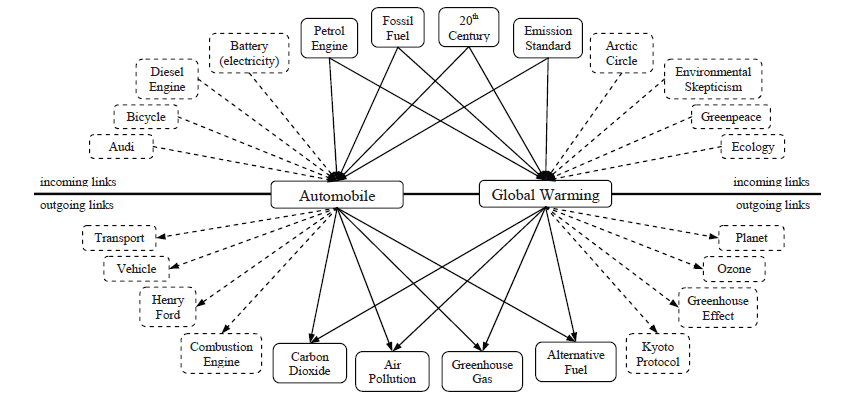
\includegraphics[width=0.7\textwidth]{images/relatedness}
 \caption{Example of relatedness between the articles \textit{Automobile} end \textit{Global Warming} (extracted from \cite{learning_link})}
 \label{fig:relatedness_example}
\end{figure*}
\paragraph{Description.}
In order to quantify the similarity between links sets, we computed three different metrics  : Jaccard coefficient, Dice\'\ s measure and Normalized Google Distance. \
These three metrics are shown in Table \ref{fig:formulas}. Given two articles $p$ and $\beta$, A and B will respectively stand for the set of articles linking (considering both incoming and outgoing links) to article $p$ and the set of articles linking to $\beta$ while W will represent the entire dataset.
\begin{table}[H]
\caption{Relatedness measure formulas and values range}
\centering
\begin{tabular}{lcc}
\toprule
Formula & Min. & Max.\\
\midrule
$Dice(p ,\beta)=2\times\frac{|A \cap B|}{|A| + |B|}$ & 0 & 1 \\
 & & \\
$Jaccard(p ,\beta)= \frac{|A\cap B|}{|A\cup B|}$ & 0 & 1 \\
 & & \\
$NGD(p ,\beta)= \frac{log(max(|A|,|B|))-log(|A\cap B|))}{log(|W|)-log(min(|A|,|B|))}$ & 0 & $\infty $ \\
\bottomrule
\label{fig:formulas}
\end{tabular}
\end{table}
Jacccard and Dice's measures are quite similar. They measure a rate of links both pages have in common.  Then they have a very intuitive meaning. The higher the measure is, the closer the topics of these articles are.

Normalized Google distance was originally based on term occurrences in web pages and it was first used by Google search engine. As explained by David Milne and Ian H. Written in their article \textit{"An Effective, Low-Cost Measure of Semantic Relatedness Obtained from Wikipedia Links"}\cite{learning_link}, this measure can also be adapted to measure relatedness between two Wikipedia articles. The smaller the distance is, the more related the articles should be. An infinite distance indicates that the two articles don't share any link. We chose to implement this possibility by replacing the infinite value by a threshold of 1000 which, compared to the highest values of the feature, seemed high enough not to distort the results.
\paragraph{Motivation.}
We chose to integrate this relatedness feature because we made the assumption that a user who is reading an article about a specific topic might be interested in reading more articles about the same domain. 
\paragraph{Extraction.}
As described before for the link position feature, links sets are extracted from the raw articles text from Wikipedia dumps. Each prominent article was attributed its own set of links. Then we computed the three metrics shown before. 

\subsection{Textual similarity}
\label{textual similarity}
\paragraph{Description.}
This feature measures the textual content similarity between two Wikipedia articles. It makes a semantic comparison between two texts and attributes a value between 0 and 1. The higher this value gets, the more similar the two articles are supposed to be.

% table has to be mentioned hear to appear in the next page
\begin{table*}[b!]
\centering
\caption{Descriptive statistics for all (non binary) features}
\label{features_stat}
\resizebox{\textwidth}{!}{%
\begin{tabular}{l
	S[table-format=1.4,
      table-figures-exponent=1,
      table-sign-mantissa,
      table-sign-exponent]
    S[table-format=1.4,
      table-figures-exponent=2,
      table-sign-mantissa,
      table-sign-exponent]
    S[table-format=1.4,
      table-figures-exponent=1,
      table-sign-mantissa,
      table-sign-exponent]
    S[table-format=1.4,
      table-figures-exponent=1,
      table-sign-mantissa,
      table-sign-exponent]
    S[table-format=1.4,
      table-figures-exponent=1,
      table-sign-mantissa,
      table-sign-exponent]
    S[table-format=1.4,
      table-figures-exponent=1,
      table-sign-mantissa,
      table-sign-exponent]
    }
\toprule
&  &  & \multicolumn{3}{c}{Quartiles} & \\
\cmidrule{4-6}
\multicolumn{1}{c}{Feature} & \multicolumn{1}{c}{Mean} & \multicolumn{1}{c}{Min.} & \multicolumn{1}{c}{$Q_1$} & \multicolumn{1}{c}{$Q_2$} & \multicolumn{1}{c}{$Q_3$} &  \multicolumn{1}{c}{Max.} \\
\midrule
Link order & 0.4651 &  0.0002 & 0.2066 & 0.4505 & 0.7126 & 1.0000\\
Link position & 0.4358 & 0.0001 & 0.1558 & 0.4034 & 0.7009 & 1.0000\\
Link order log & 0.8185 & 0.0000 & 0.7466 & 0.8720 & 0.9459 & 1.0000\\
Link position log & 0.8858 & 0.2300 & 0.8382 & 0.9209 & 0.9690 & 1.0000 \\  
Link count & 1.4796 & 1.0000 & 1.0000 & 1.0000 & 1.0000 & 255.0000 \\
Hubs score & 3.4345e-5 & 8.3122e-19 & 1.1513e-8 & 7.7927e-8 & 5.0804e-7 & 1.0000\\ 
Authority score & 9.9120e-5 & 1.7678e-15 & 1.0063e-09 & 4.1116e-9 & 2.0688e-8 & 1.0000\\
Page rank & 9.0000e-5 & 1.0000e-6 & 2.0000e-6 & 4.0000e-6 & 1.1000e-5 & 1.9789e-2\\
Title similarity & 0.0225 & 0.0000 & 0.0000 & 0.0000 & 0.0000 & 0.8750\\
Search interest & 0.6130 & 0.0000 & 0.5038 & 0.6301 & 0.7381 & 1.0000\\
Social interest & 0.2194 & 0.0000 & 0.0000 & 0.0000 & 0.4165 & 1.0000\\ 
Social interest 2 & 0.1879 & 0.0000 & 0.0000 & 0.0000 & 0.3084 & 1.0000\\ 
Search interest 2 & 0.4872 & 0.0000 & 0.2306 & 0.4870 & 0.7405 & 1.0000\\ 
Jaccard coeff. & 0.0050 & 0.0000 & 0.0000 & 0.0000 & 0.0048 & 0.4545 \\
Dice coeff. & 0.0095 & 0.0000 & 0.0000 & 0.0000 & 0.0094 & 0.6200 \\
Google distance & 547.6310 & 0.0823 & 0.5444 & 1000.0 & 1000.0 & 1000.0\\
Text similarity & 0.6261 & 0.0000 & 0.5170 & 0.6840 & 0.7890 & 0.9900\\

\bottomrule
\end{tabular}
}
\end{table*}

\paragraph{Motivation.}
The idea behind this feature is that two articles containing approximately the same words are likely to discuss closely related subjects. This is another way to know how the two articles are related on a more semantic level than the relatedness feature we described before.

\paragraph{Extraction.}
The text of all articles is extracted from wikipedia dumps. We get rid of all non-text information (tables, url links, etc ...) with regular expressions.

Then, for both articles $p$ and $\beta$ we create a vector that describe the frequencies of the relevant words (TF-IDF vector).

Finally the method compares the frequencies of relevant words between article $p$ and article $\beta$ by using the cosine of these two vectors.

\subsection{Title similarity}
\label{title similarity}
Using similarity between titles as a feature is motivated by e.g. the observation that articles on people often have their family members among the most popular reference links and these often share family name whereas we would observe a higher title similarity. Similarly, a movie in a series often has e.g. its prequels/sequels highly ranked.

The feature was implemented using Jaccard similarity of the title words. %We achieved a correlation coefficient of $r = 0,0115$.

